%%%%%%%%%%%%%%%%%%%%%%%%%%%%%%%%%%%%%%%%%%%%%%%%%%%%%%%%%%%%%%%%%%%%%
%
%  This is a sample LaTeX input file for your contribution to 
%  the MC2013 conference. Modified by R.C. Martineau at INL from A. 
%  Sood at LANL, from J. Wagner ORNL who obtained the original class 
%  file by Jim Warsa, LANL, 16 July 2002}
%
%  Please use it as a template for your full paper 
%    Accompanying/related file(s) include: 
%       1. Document class/format file: mc2013.cls
%       2. Sample Postscript Figure:   figure.eps
%       3. A PDF file showing the desired appearance: template.pdf 
%    Direct questions about these files to: richard.martinea@inl.gov
%
%    Notes: 
%      (1) You can use the "dvips" utility to convert .dvi 
%          files to PostScript.  Then, use either Acrobat 
%          Distiller or "ps2pdf" to convert to PDF format. 
%      (2) Different versions of LaTeX have been observed to 
%          shift the page down, causing improper margins.
%          If this occurs, adjust the "topmargin" value in the
%          mc2013.cls file to achieve the proper margins. 
%
%%%%%%%%%%%%%%%%%%%%%%%%%%%%%%%%%%%%%%%%%%%%%%%%%%%%%%%%%%%%%%%%%%%%%


%%%%%%%%%%%%%%%%%%%%%%%%%%%%%%%%%%%%%%%%%%%%%%%%%%%%%%%%%%%%%%%%%%%%%
\documentclass{mc2013}
%
%  various packages that you may wish to activate for usage 
\usepackage{graphicx}
\usepackage{tabls}
\usepackage{afterpage}
\usepackage{cites}
%\usepackage{epsf}
%
%
% Insert authors' names and short version of title in lines below
%
\newcommand{\authorHead}      % Author's names here
   {Slattery, Wilson, and Pawlowski}  
\newcommand{\shortTitle}      % Short title here
   {Data Transfer Kit}  
%%%%%%%%%%%%%%%%%%%%%%%%%%%%%%%%%%%%%%%%%%%%%%%%%%%%%%%%%%%%%%%%%%%%%
%
%   BEGIN DOCUMENT
%
%%%%%%%%%%%%%%%%%%%%%%%%%%%%%%%%%%%%%%%%%%%%%%%%%%%%%%%%%%%%%%%%%%%%%
\begin{document}

%
%      Headers and Footers
\afterpage{%
\fancyhf{}%
\fancyhead[CE]{              
{\scriptsize \authorHead}}                                                
\fancyhead[CO]{               
{\scriptsize \shortTitle}}                  
%\lfoot{\scriptsize{
%International Conference on Mathematics and Computational Methods
%Applied to Nuclear Science \& Engineering (M\&C 2013), 
%\\ Sun Valley, Idaho, USA, May 5-9, 2013.}}%
\rfoot{\thepage/\totalpages{}}%

\pagestyle{fancy}
%\setlength{\topmargin}{-20pt}
}
 
\normalsize

\setlength{\baselineskip}{16.8pt}
\vspace{-3pt}

% 
% TITLE
%

\begin{center}
\textbf{\large \\%
THE DATA TRANSFER KIT: A GEOMETRIC RENDEZVOUS-BASED TOOL FOR
MULTIPHYSICS DATATRANSFER
}
% 
% FIRST AUTHORS 
%
\\
\setlength{\baselineskip}{14pt}
\textbf{S.R. Slattery and P.P.H. Wilson} \\
Department of Engineering Physics \\
University of Wisconsin - Madison \\
1500 Engineering Dr., Madison, WI 53706 \\
sslattery@wisc.edu; wilsonp@engr.wisc.edu \\

% 
% SECOND AUTHORS (if not needed delete from here) 
%
\vspace{12pt}
\textbf{R.P. Pawlowski}\\
Sandia National Laboratories \\
1515 Eubank SE, Albuquerque, NM 87123 \\
rppawlo@sandia.gov \\ 
%
% SECOND AUTHORS (to here)
%

\end{center}

%
% SET RAGGED RIGHT MARGIN
%
\raggedright


%%---------------------------------------------------------------------------%%
\section*{ABSTRACT} 
\begin{quote}
\begin{small}
The Data Transfer Kit (DTK) is a software component designed to
provide parallel services for mesh searching and data transfer for
arbitrary physics components based on the concept of geometric
rendezvous. The rendezvous algorithm provides a means to geometrically
correlate two meshes that may be arbitrarily decomposed in a parallel
simulation. By repartitioning both meshes such that they have the same
geometric domain on each parallel process, efficient and load balanced
search operations and field evaluations can be performed at a
desirable algorithmic time complexity with low communication overhead
relative to other types of mapping algorithms. With the increased
development efforts in multiphysics simulation, adaptive mesh
simulations, and other multiple mesh problems, generating parallel
topology maps for transferring fields and other data between meshes is
a common operation. This document describes the algorithms to generate
parallel topology maps based on the concept of geometric rendezvous as
implemented in DTK with examples using the Drekar CFD code a surrogate
neutronices code and gives the results of initial scaling studies
performed on the Jaguar system at Oak Ridge National Laboratory for a
simplified problem.


\emph{Key Words}: data transfer, multiphysics, rendezvous, parallel
\end{small} 
\end{quote}

\setlength{\baselineskip}{14pt}
\normalsize

%%---------------------------------------------------------------------------%%
\Section{INTRODUCTION} 
\label{sec:intro}

In many physics applications, it is often desired to transfer fields
(i.e. degrees of freedom or other data) between meshes that may or may
not conform in physical space. In addition, for massively parallel
simulations, it is typical that meshes not only do not conform
spatially, but also that their parallel decompositions do not
correlate and are independent of one another due to physics-based
partitioning and discretization requirements. As an example, this
situation can occur in multiphysics simulations where physics fields
provide feedback between solution iterations or adaptive mesh
simulations where fields must be moved between meshes after refining
and coarsening. It is therefore desirable to have a set of tools to
relate two meshes of arbitrary parallel decomposition such that fields
and other data can be transferred between them.

The Data Transfer Kit (DTK) is a software component devloped as part
of the Consortium for Advanced Simulation of LWR's (CASL) designed to
provide parallel services for mesh searching and data transfer based
on the concept of the rendezvous decomposition as developed by
Plimpton, Stewart, and Hendrickson \cite{Plimpton_2004}. To achieve a
component design for use with arbitrary physics codes, general
concepts of mesh and fields are employed to provide access to these
services. This document will outline the concepts of parallel
communicators, mesh, fields, parallel topology maps, and the
rendezvous decomposition and how they are modeled within the design of
DTK. An example of data transfer using these concepts is also
provided.


%%---------------------------------------------------------------------------%%
\Section{RENDEZVOUS ALGORITHMS} 
\label{sec:rendezvous_algorithms}

%%---------------------------------------------------------------------------%%
\Section{NEUTRONICS-CFD COUPLING EXAMPLE}
\label{sec:neutronics_cfd}

%%---------------------------------------------------------------------------%%
\Section{SCALING STUDY}
\label{sec:scaling_study}

A typical use case of DTK is searching a mesh with a set of points and
applying field data to those points. For this use case, a scaling
study of the initial DTK implementation of the rendezvous algorithm
for data transfer was performed utilizing the Jaguar system. For each
study, a tri-linear hexahedron mesh was generated and decomposed
across the parallel domain. Figure~\ref{fig:mesh_partition} shows an
example of a mesh partition used in the scaling studies. Each
partition had one element in the z direction while the x and y
directions were varied to produce the desired number of elements in
the partition. All partitions in each scaling study are square. This
mesh is searched with random points generated by sampling the x and y
directions across the global mesh domain.  By striding the random
number seed used to generate the point coordinates, each process will
have a unique set of random points it is searching for. For each
scaling study, every process generated the same number of random
points as the number of elements on that process, ensuring that a
dense, all-to-all communication operation will be required for mapping
and data transfer. Once the points are mapped to the mesh, the data
transfer routine applies the process rank in which they were found and
transfers it back to the original owning process for the point. In
this way, because of the simple partitioning used for the scaling
studies, the results of the data transfer to the random points can be
independently verified by checking the applied data against the
expected mesh process rank.

\begin{figure}[htpb!]
  \centering 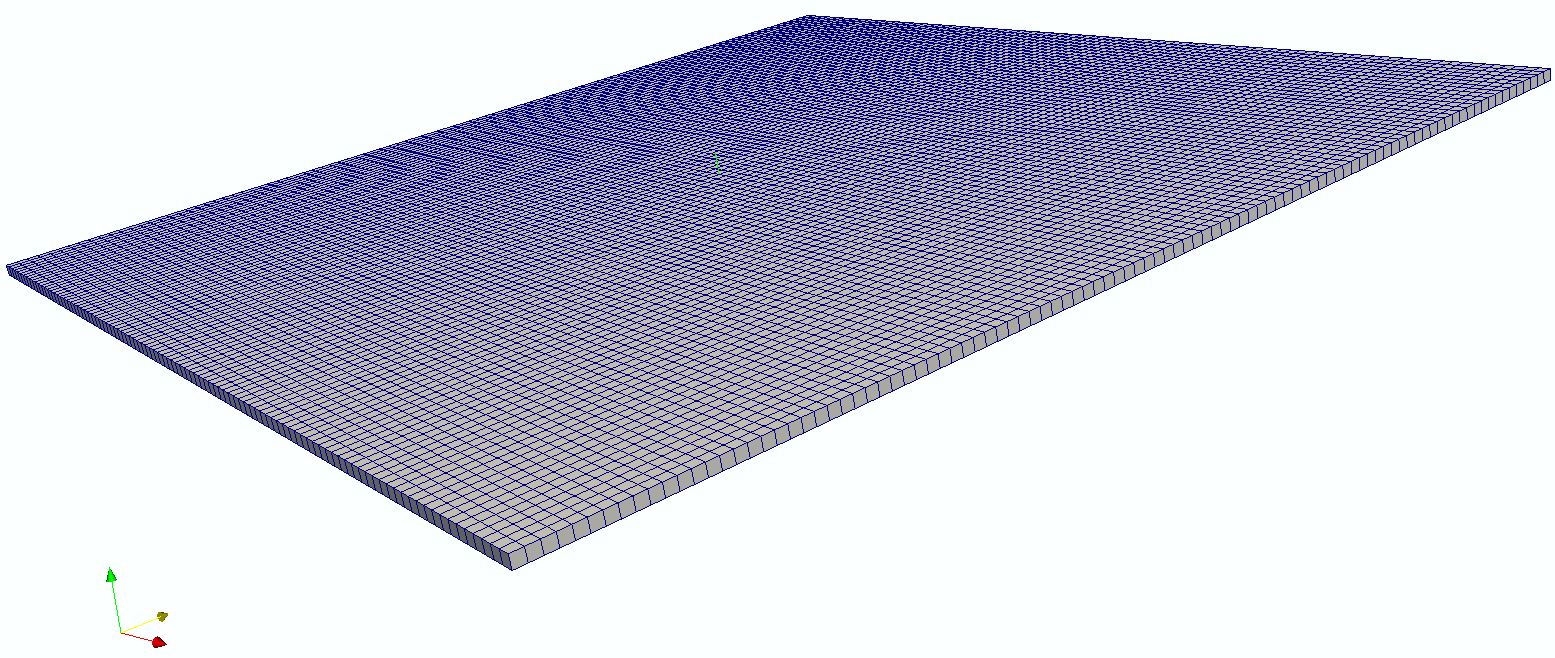
\includegraphics[width=5.5in]{mesh.png}
  \caption{\sl Local mesh partition for scaling studies. This
    particular mesh partition has 1.0E4 tri-linear hexahedrons.}
  \label{fig:mesh_partition}
\end{figure}

Three scaling variations were investigated. A weak scaling study was
performed by fixing the problem size per core and increasing the
number of cores used. A strong scaling study was performed by fixing
the total problem size while increasing the number of cores
used. Finally, a study where the number of cores was fixed while
increasing the total problem size per core was also investigated.


%%---------------------------------------------------------------------------%%
\Section{CONCLUSIONS}

Initial scaling studies have been completed for the Data Transfer Kit
on the Jaguar system. Their results show comparable qualitative
behavior to the literature results with improved performance due to
the more advanced computational resources available. Implementation
improvements have made significant gains in performance, however, for
the dense communication patterns required to complete the scaling
study problem, poor scaling results are still observed above O(10,000)
processors. It is expected for more physical data transfer problems
that the communication pattern will be significantly sparser than the
problem presented here. Because of this, scaling is expected to
improve for more physical problems. Additional scaling studies will be
required to test this hypothesis.


%%---------------------------------------------------------------------------%%
\section*{ACKNOWLEDGEMENTS}

This work was performed under funding provided by the Consortium for
Advanced Simulation of Light Water Reactors (CASL).

%%---------------------------------------------------------------------------%%
%\Section*{REFERENCES}
\setlength{\baselineskip}{12pt}
\bibliography{references}

\end{document}


